\documentclass[a4paper]{article}
\usepackage[UTF8]{ctex}
\usepackage{geometry}
\usepackage{graphicx}
\usepackage{url}
\usepackage{multirow}
\usepackage{array}
\usepackage{booktabs}
\usepackage{url}
\usepackage{enumitem}
\usepackage{graphicx}
\usepackage{float}
\usepackage{amssymb}
\usepackage{amsmath}
\usepackage{subfig}
\usepackage{longtable}
\usepackage{pifont}
\usepackage{color}
\usepackage{listings}
\usepackage{xcolor}

\allowdisplaybreaks

\geometry{a4paper, scale=0.78}

% \begin{figure}[H]
%     \centering
%     \includegraphics[width=.55\textwidth]{E.png}
%     \caption{矩阵与列向量的乘法}
%     \label{fig:my_label_1}
% \end{figure}

% \left\{
% \begin{array}{ll}
%       x+2x+z=2 & \\
%       3x+8y+z=12 & \\
%       4y+z=2
% \end{array}
% \right.

% \begin{enumerate}[itemindent = 1em, itemsep = 0.4pt, parsep=0.5pt, topsep = 0.5pt]

% \end{enumerate}

%\stackrel{a}{\longrightarrow}

\title{Kernel Method 01 Background}
\author{Chen Gong}
\date{20 November 2019}

\begin{document}
\maketitle

在Support Vector Machine的章节中,我们已经分析了支持向量机前面“两宝”,也就是间隔和对偶,而第三宝,核技巧在这里我们需要抽出来将分析。其实,我最开始学习核的时候,真的是一脸懵逼,这玩意到底是个什么鬼?来龙去脉是什么?这这节有关于Kernel Method的背景介绍中,我想分析一下,我们为什么要使用核?以及怎么用核?来给大家一个直观的感受。

本小节主要从Kernel Method,Kernel Function和Kernel Trick,三个方面来进行分析和讨论,我们为什么要用核?我们怎么样用核?

\section{Kernel Method}
核方法是一种思想,在Cover Theorem中提出:高维空间比低维空间更容易线性可分。这句话非常的直观,我们想想就理解了,这里我不做出详细的证明。在这里我们举一个例子,对于经典的线性不可分问题异或问题,图像描述如下所示:
\begin{figure}[H]
    \centering
    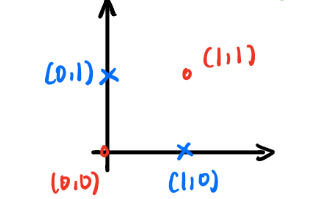
\includegraphics[width=.5\textwidth]{微信图片_20191120100717.png}
    \caption{异或问题的图像在二维空间中的描述}
    \label{fig:my_label_1}
\end{figure}

这二维空间中的点可以被我们记为$X=(x_1,x_2)$,如果我们使用一个变换函数,将其变换到三维空间中就会发生有意思的事情。我们设定一个变换函数为$\phi(X)$,将二维空间中的点,变换到一个三维空间$Z$中,并且令$Z=(x_1,x_2,(x_1-x_2)^2)$,那么我们再来看看异或问题在三维空间中点的分布,我们惊奇的发现变得线性可分了:
\begin{figure}[H]
    \centering
    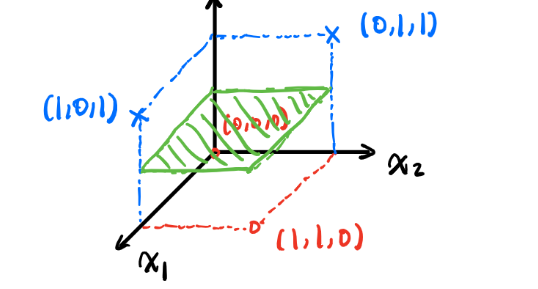
\includegraphics[width=.7\textwidth]{微信图片_20191120101440.png}
    \caption{异或问题的图像在三维空间中分布}
    \label{fig:my_label_2}
\end{figure}

通过这个例子,想想大家都直观的感受到了高维空间带来的好处。实际上对于解决非线性问题,我们有两种思路:

1. 也就是之前提到的,由Perceptron Layer Analysis (PLA) 引出的多层感知机 (Multilayer Perceptron)也就我们经常听到的神经网络,以及之后发展得到的Deep Learning。

2. 而第二种思路就是通过非线性变换$\phi(x)$,将非线性可分问题转换为线性可分问题。上述的异或问题,可以表述为:
\begin{equation}
    \mathcal{X}=(x_1,x_2) \stackrel{\phi(x)}{\longmapsto} \mathcal{Z}=(x_1,x_2,(x_1-x_2)^2)
\end{equation}

第二类方法也就是我们讨论的重点,其实在我们机器学习理论的研究中,第二种方法有很大的威力,大部分同学在学习的时候都会忽掉,例子可以看看之前发的再生核希尔伯特空间。

\section{Kernel Function}
核函数,从模型的角度讲可以带来给非线性带来高维的转换,这个我们上面已经分析过了。从优化的角度讲可以为对偶带来内积,这两个角度可以合在一起看看。

以我们之前学习的Hard Margin SVM为例,原问题和对偶问题的表述为:
\begin{equation}
    \begin{split}
        &\left\{
        \begin{array}{ll}
        \max_{w,b} \ \frac{1}{2} w^Tw & \\
        s.t. \quad 1-y_i(w^T_ix+b)\leq 0  & \\
        \end{array}
    \right. \\
    & \left\{
    \begin{array}{ll}
          \min_\lambda \frac{1}{2}\sum_{i=1}^N\sum_{j=1}^N\lambda_i\lambda_jy_iy_j(x_i^Tx_j) - \sum_{i=1}^N\lambda_i & \\
          s.t.\quad \ \lambda_i \geq 0,\ \sum_{i=1}^N \lambda_iy_i = 0  & \\
    \end{array}
    \right.
    \end{split}
\end{equation}

在我们的对偶问题中,是不是有一个$x_i^Tx_j$。在线性可分问题中,我们直接计算就好了,在线性不可分问题中,就需要将$x$通过一个变换$\phi$转换到高维空间中。那么$x_i^Tx_j$就变成了$\phi(x_i^T)\phi(x_j)$。那么我们就将两个角度的分析联系起来了。那么核函数我们可以定义为:

对于一个$K(x,x')=\phi(x)^T\cdot\phi(x)=<\phi(x),\phi(x')>$,

有$\forall x,x' \in \mathcal{X},\exists\phi:x\mapsto z \ s.t. \ K(x,x') = \phi(x)^T\cdot \phi(x')$。则称$K(x,x')$是一个核函数。比如:
\begin{equation}
    K(x,x')=exp(-\frac{(x-x')^2}{2\sigma^2})
\end{equation}

\section{Kernel Track}
下面我们需要引入核技巧了,也就是想想,核函数有什么用?前面我们讲到将$x$通过一个变换$\phi$转换到高维空间。但是,有可能$\phi(x)$的维度非常的高,甚至是无限维的,那么这将变得非常的难求。如果还要继续求$\phi(x_i^T)\phi(x_j)$,这个计算量恐怕会要原地爆炸。

大家通过上面的表达会发现我们实际上关注的不是$\phi(x_i)$本身,而是$\phi(x_i^T)\phi(x_j)$。那么,我们完全可直接求跳过求$\phi(x_i)$的过程,然后$\phi(x_i^T)\phi(x_j)$。我们看看核函数的定义,是不是$K(x_i,x_j)$就等于$\phi(x_i^T)\phi(x_j)$。这就省去了很多麻烦的计算过程,核函数在这实在是太好用了,这就是核技巧的思想。总的来说,就是非线性转换上的一个内积。
~\\

我们为什么引入kernel?就是原来的方法有不足,不能解决非线性可分问题。所以,我们想到利用核函数将$\mathcal{X}\mapsto\mathcal{Z}$,到更高维的空间来转换成线性可分问题。又因为$\phi(x_i)$的计算很难,我们有想到用核函数来直接求$\phi(x_i^T)\phi(x_j)$。这里面其实是一环扣一环的,逻辑性非常的强。

对于前面讨论的线性可分问题Perceptron Layer Analysis和Hard Margin SVM。允许出现错误就出现了Pocket Algorithm和Soft Margin SVM。进一步如果是严格的非线性问题,引入了$\phi(x)$就得到了$\phi(x)+PLA$
和$\phi(x)+Hargin$ (Kernel SVM),就是将输入变量的内积转换为核函数。

那么,我们怎么找一个核函数,核函数具有怎样的性质?我们在下一小节中进行分析。





\end{document}
